% =====================================================================
% CASPT & TransitData 2027 -- research track (regular paper, max 8 pages)
% Preamble = official CASPT2027_LaTeX_template.tex preamble, kept verbatim.
% Every deviation from the template is tagged "CASPT-ADAPT".
% Content: condensed from the WCTR 2026 manuscript in res/WCTR2026/.
% =====================================================================
% Options for packages loaded
\PassOptionsToPackage{unicode}{hyperref}
\PassOptionsToPackage{hyphens}{url}
\documentclass[11pt]{article}  % Set the document class to 11pt
\usepackage{longtable}
\usepackage{array}
\usepackage{caption} % Required for customizing captions
\captionsetup{labelfont={bf}, font={small, bf}, skip=0pt} % Customize caption font% for defining custom column types
\usepackage{booktabs} % for nicer horizontal rules
\usepackage{amsmath,amssymb}
\usepackage{lmodern}
\usepackage{iftex}
\ifPDFTeX
  \usepackage[T1]{fontenc}
  \usepackage[utf8]{inputenc}
  \usepackage{textcomp} % provide symbols
\else % if luatex or xetex
  \usepackage{unicode-math}
  \defaultfontfeatures{Scale=MatchLowercase}
  \defaultfontfeatures[\rmfamily]{Ligatures=TeX,Scale=1}
\fi

% use natbib with apa style for automatic reference handling
\usepackage[style=apa,natbib=true]{biblatex}
\bibliography{bibliography}

% Use upquote if available, for straight quotes in verbatim environments
\IfFileExists{upquote.sty}{\usepackage{upquote}}{}
\IfFileExists{microtype.sty}{% use microtype if available
  \usepackage[]{microtype}
  \UseMicrotypeSet[protrusion]{basicmath} % disable protrusion for tt fonts
}{}
\makeatletter
\@ifundefined{KOMAClassName}{% if non-KOMA class
  \IfFileExists{parskip.sty}{%
    \usepackage{parskip}
  }{% else
    \setlength{\parindent}{0pt}
    \setlength{\parskip}{6pt plus 2pt minus 1pt}}
}{% if KOMA class
  \KOMAoptions{parskip=half}}
\makeatother
\usepackage{xcolor}
\usepackage{longtable,booktabs,array}
\usepackage{calc} % for calculating minipage widths
% Correct order of tables after \paragraph or \subparagraph
\usepackage{etoolbox}
\makeatletter
\patchcmd\longtable{\par}{\if@noskipsec\mbox{}\fi\par}{}{}
\makeatother
% Allow footnotes in longtable head/foot
\IfFileExists{footnotehyper.sty}{\usepackage{footnotehyper}}{\usepackage{footnote}}
\makesavenoteenv{longtable}
\usepackage{graphicx}
\makeatletter
\def\maxwidth{\ifdim\Gin@nat@width>\linewidth\linewidth\else\Gin@nat@width\fi}
\def\maxheight{\ifdim\Gin@nat@height>\textheight\textheight\else\Gin@nat@height\fi}
\makeatother
% Scale images if necessary, so that they will not overflow the page
% margins by default, and it is still possible to overwrite the defaults
% using explicit options in \includegraphics[width, height, ...]{}
\setkeys{Gin}{width=\maxwidth,height=\maxheight,keepaspectratio}
% Set default figure placement to htbp
\makeatletter
\def\fps@figure{htbp}
\makeatother
\setlength{\emergencystretch}{3em} % prevent overfull lines
\providecommand{\tightlist}{%
  \setlength{\itemsep}{0pt}\setlength{\parskip}{0pt}}
% CASPT-ADAPT: the template disables automatic numbering and types the numbers
% by hand ("\section{1. Introduction}"). We keep automatic numbering so that the
% \ref cross-references of the original manuscript keep working, and print the
% numbers in the template's style ("1. Introduction", "3.1 Subsections").
%\setcounter{secnumdepth}{-\maxdimen} % remove section numbering
\setcounter{secnumdepth}{3}
\makeatletter
\def\@seccntformat#1{\csname the#1\endcsname\csname caspt@suffix@#1\endcsname\ }
\def\caspt@suffix@section{.}
\makeatother
\ifLuaTeX
  \usepackage{selnolig}  % disable illegal ligatures
\fi
\IfFileExists{bookmark.sty}{\usepackage{bookmark}}{\usepackage{hyperref}}
\IfFileExists{xurl.sty}{\usepackage{xurl}}{} % add URL line breaks if available
\urlstyle{same} % disable monospaced font for URLs

\author{}
\date{}

% CASPT-ADAPT: the template instructions require ISO A4; "a4paper" is stated
% explicitly so the page size does not depend on the local TeX default.
\usepackage[a4paper,margin=25mm]{geometry}

% For Times New Roman font
\usepackage{mathptmx} % Use the mathptmx package to set the font to Times New Roman

% If you need to use the T1 encoding for better font support, include this package
\usepackage[T1]{fontenc}

% =====================================================================
% CASPT-ADAPT: packages and macros needed by the content of this paper
% (carried over from the original manuscript preamble).
% =====================================================================
\usepackage{tabularx}
\usepackage{multirow}
\DeclareMathAlphabet{\pazocal}{OMS}{zplm}{m}{n}
\newcolumntype{Y}{>{\centering\arraybackslash}X}
% The original manuscript uses natbib (authoryear), where \citet is narrative
% and \citep parenthetical; biblatex (natbib=true) provides both.
\providecommand{\sep}{\unskip; }

\begin{document}

{\centering

{\fontsize{16}{16} % Adjust the size of the font according to the guideline 
\selectfont
\textbf{\textsc{Proactive--Adaptive Public Transport Planning: Bus Network Redesign for Urban Rail Disruptions}}}

\vspace{16pt} % Adjust the spacing as needed

Zihao GUO\textsuperscript{1,*}, Andrea ARALDO\textsuperscript{1}, Moun\^{i}m A. EL YACOUBI\textsuperscript{1}

\textit{\textsuperscript{1}SAMOVAR, T\'el\'ecom SudParis, Institut Polytechnique de Paris, Palaiseau 91120, France; zihao-eric.guo@ip-paris.fr, andrea.araldo@telecom-sudparis.eu, mounim.el\_yacoubi@telecom-sudparis.eu}

* Corresponding author

\vspace{12pt} % Adjust the spacing as needed

\emph{Regular paper submitted for presentation at International Conference
on Advanced Systems in Public Transport and TransitData 2027}

\emph{June 21-24, 2027, Stockholm, Sweden}

\vspace{12pt} % Adjust the spacing as needed

}

\textbf{Abstract}: Accessibility, understood as the extent to which opportunities can be reached within a specified travel-time threshold, constitutes a central benefit of public transport systems. Although Urban Rail Transit (URT) plays a pivotal role in ensuring such accessibility, its inherent susceptibility to disruptions disproportionately affects suburban regions where alternative travel options are scarce. Existing disruption management strategies, however, often fall short: rigid proactive measures offer limited operational flexibility, whereas purely reactive responses are typically inefficient in restoring accessibility once disruptions occur. To address these limitations, this paper introduces a two-stage stochastic optimization framework that couples proactive infrastructure investment with adaptive operational adjustments. The first stage identifies flexible network enhancements to be implemented in advance, while the second stage optimizes bus operations in response to disruption scenarios. Results from a stylized case study reveal that, relative to conventional replacement buses, the proposed framework consistently achieves higher accessibility restoration across disruption scenarios, while maintaining at least 66.7\% path similarity with the original bus routes.

\textbf{Keywords}: Proactive-adaptive strategy \sep Accessibility \sep Public transport resilience \sep Disruption management \sep Two-stage stochastic programming

\_\_\_\_\_\_\_\_\_\_\_\_\_\_\_\_\_\_\_\_\_\_\_\_\_\_\_\_\_\_\_\_\_\_\_\_\_\_\_\_\_\_\_\_\_\_\_\_\_\_\_

% =============================================
\section{Introduction}\label{sec:intro}
% =============================================
Urban Rail Transit (URT) systems form the backbone of metropolitan mobility, providing high-capacity, reliable services under normal operations~\citep{tan2020evacuating}. Yet this critical infrastructure remains vulnerable to diverse disruptions, from unexpected incidents to planned maintenance: a fire at New York City's 145th Street Station suspended service for over two hours during the morning peak~\citep{barone2017abcdfire}, recurring closures on Paris's RER B line have affected nearly 200,000 daily passengers despite replacement bus deployments~\citep{actu2024travaux}, and even the highly reliable Hong Kong MTR experiences hundreds of disruptions per year~\citep{zhang2020metro}.

The fallout from URT disruptions signifies more than mere delays; it represents a critical failure of access. Although city centers may have redundant routes, suburbs with thinner networks are far more vulnerable: a single disruption there can cut people off from vital destinations such as jobs, schools, or hospitals~\citep{liu2024measuring}. Traditional metrics like average delay therefore provide an incomplete picture. A more comprehensive metric is \emph{accessibility}, the practical ability to reach important daily destinations within a reasonable time~\citep{hansen1959accessibility,miller2020measuring}.

Current disruption management tools are not well-equipped to protect that kind of access. The go-to solution, substitute buses along the affected rail corridor (\emph{bus bridging}), tends to recreate the form of service without delivering its function~\citep{Pender2012,CurrieMuir2017}: replacement buses often suffer from inadequate capacity, longer travel times, and poor reliability compared to the original rail system~\citep{CurrieMuir2017}. More generally, the literature has followed two largely separate streams. \emph{Proactive} planning strengthens the network before disruptions occur, e.g., through redundant routes or vulnerability and resilience analysis~\citep{CatsJenelius2014,RodriguezNunez2014,XuChopra2022}; these approaches are inherently static, often conservative, and frequently remain at an analytical level. \emph{Reactive} operations, such as train rescheduling~\citep{Cacchiani2014}, bus bridging route design and dispatching~\citep{Jin2016,vanDerHurk2016}, stop skipping~\citep{Tang2018}, or short turning~\citep{Peled2021} (see~\citealp{Gkiotsalitis2022}, for an overview), are applied after a disruption occurs; they are generally ad hoc, tailored to specific cases, and optimize local performance rather than system-wide outcomes. Stochastic and robust models that integrate design and operations exist~\citep{Cadarso2015,AnLo2016}, but strategic infrastructure planning and operational disruption management are still mostly treated separately~\citep{Besinovic2020}. Moreover, while accessibility is well established in transport planning~\citep{geurs2004accessibility}, URT disruption research has used it to \emph{measure} disruption impacts~\citep{liu2024measuring,nalin2025evaluation} but not as an \emph{optimization objective} for recovery.

To address this gap, we propose a bus network redesign methodology for URT disruptions that jointly integrates preventive planning and adaptive operations, with accessibility as the explicit objective. We formulate a two-stage stochastic program: in the first stage, candidate stops, dedicated bus lanes and contingency line topologies are prepared before any disruption; in the second stage, service frequencies and passenger routings are adapted to the realized disruption scenario. A Path Order Preservation Rate (POPR) constraint keeps redesigned lines close to their original structure, limiting passenger disorientation and driver operational complexity. On a stylized case study, the framework consistently outperforms conventional replacement buses in accessibility while maintaining at least 66.7\% path similarity.

% =============================================
\section{Problem Setting}\label{sec:preliminaries}
% =============================================
The system is defined as a 4-tuple $\Sigma = (\pazocal{S}, \pazocal{G}, \pazocal{L}, \Omega)$, where $\pazocal{S}$ is the spatial tessellation of the study area, $\pazocal{G}$ the physical infrastructure graph, $\pazocal{L}$ the set of PT service lines, and $\Omega$ the set of disruption scenarios.

\textbf{Tessellation and demand.} We partition the study area into a regular tessellation of tiles $s \in \pazocal{S}$ with centroids $c_s$. A traveler can either walk directly or combine walking with PT. Walking times $\bar{t}_{sj}^{\text{access}}$ from $c_s$ to each stop $j$ are precomputed; tiles without stops are assigned a candidate stop at $c_s$. For each tile $s$, $\pazocal{O}_s$ is the set of activity opportunities (workplaces, schools, healthcare facilities) linked to $s$. The pair $(s,k)$, $k \in \pazocal{O}_s$, is referred to as an origin--destination (OD) pair.

\textbf{Network graph.} The PT network is a directed multi-layer graph $\pazocal{G} = (\pazocal{N}, \pazocal{E})$. The node set $\pazocal{N} = \pazocal{N}^r \cup \pazocal{N}^b \cup \pazocal{N}^c$ consists of urban rail stations, existing bus stops and candidate bus stops. The edge set $\pazocal{E} = \pazocal{E}^r \cup \pazocal{E}^b \cup \pazocal{E}^c \cup \pazocal{E}^t$ includes rail links with travel times $\bar{t}_{ij}^r$, existing bus links, potential new bus links connecting candidate stops, and walking transfer edges with times $\bar{t}_{ij}^{\text{transfer}}$. Each physical link is represented by two opposite arcs.

\textbf{Service layer.} Urban rail lines $\pazocal{L}^r$ run on fixed routes and timetables, providing the stable backbone of the network (average waiting time $\bar{w}_i^r$ at station $i$). Bus lines $\pazocal{L}^b$ are more flexible: they can be rerouted or extended to candidate stops when rail disruptions occur. Each line is a directed simple path; the opposite direction mirrors it with the same frequency (symmetric service).

\textbf{Disruption scenarios.} Uncertainty is described by a finite set of scenarios $\Omega$. Each $\omega \in \Omega$ occurs with probability $p_\omega$ and specifies (i) rail link failures $\bar{d}_{ij}^{\omega} \in \{0,1\}$, $(i,j) \in \pazocal{E}^r$, and (ii) scenario-dependent bus travel times. Since displaced rail demand adds pressure on the road network, the nominal bus time $\bar{t}_{ij}^\ell$ of line $\ell$ on edge $(i,j)$ is inflated as $\hat{t}_{ij}^{\ell,\omega} = \bar{t}_{ij}^\ell \big(1 + \mu_{\text{bus}} \sum_{(m,n)\in \pazocal{E}^r} \bar{d}_{mn}^\omega \big)$, where the sensitivity $\mu_{\text{bus}}$ is informed by congestion multipliers of up to 2.0 reported for degraded road conditions~\citep{dft2018congestion}. Dedicated bus lanes shorten travel times by a factor $\alpha$, about 18\% on average~\citep{russo2022buslane}.

% =============================================
\section{Methodology}\label{sec:methodology}
% =============================================
\subsection{Two-stage decision process}\label{subsec:problemStatement}
Decisions operate on two time scales (Fig.~\ref{fig:PT_repre}). \emph{First-stage (here-and-now) design decisions}, taken before any disruption materializes, comprise (a) the construction of candidate stops ($z_i$), (b) the installation of dedicated bus lanes ($b_{ij}$), a tactical investment justified because it is decided once and benefits all future scenarios, and (c) the contingency topology of each bus line ($x_{ij}^\ell$), prepared in advance so that it can be activated immediately. \emph{Second-stage (recourse) decisions}, taken after scenario $\omega$ is realized, comprise (d) the service frequency $f^{\ell,\omega}$ of each line, which implicitly allocates the bus fleet, and (e) the resulting passenger routings $y_{ij}^{sk\omega}$. Disrupted rail stations are deactivated, and their passengers are directed (through phone alerts or station signage) to redesigned bus services at designated consolidation nodes. Real-time driver guidance through onboard consoles or tablets allows drivers to follow the pre-computed contingency routes with minimal additional hardware or training.

\begin{figure}[htbp]
\centering
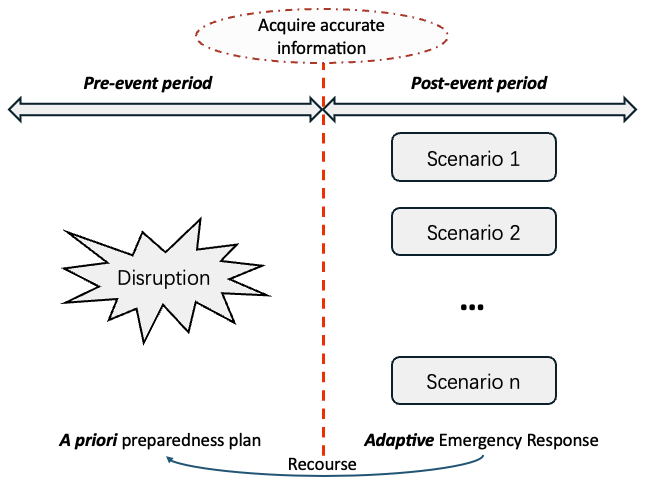
\includegraphics[width=.5\textwidth]{Figure/framework.png}
\caption{Two-stage framework for preparedness and adaptive response under disruptions. Left of the dashed boundary, first-stage design decisions ($z_i$, $b_{ij}$, $x_{ij}^\ell$) are fixed before uncertainty is resolved; to its right, second-stage recourse decisions ($f^{\ell,\omega}$, passenger routings) are taken per realized scenario.}\label{fig:PT_repre}
\end{figure}

\subsection{Performance measures}\label{subsec:measures}
\textbf{Path Order Preservation Rate (POPR).}\label{subsec:porp} Let the original route be the node sequence $P = [v_1, \dots, v_n]$ with consecutive pairs $\pazocal{S}_{\text{orig}} = \{(v_i, v_{i+1}) \mid 1 \leq i \leq n-1\}$, and $P'$ the redesigned route. A pair is preserved if $P'$ contains $(v_i,v_{i+1})$ or $(v_{i+1},v_i)$; with $K$ preserved pairs, $\text{POPR}(P,P') = K/(n-1)$. POPR is a discrete, topology-oriented counterpart of the path overlap ratio~\citep{Lim2005PathOverlap}: it keeps redesigned lines close to their original topology, mitigating passenger disorientation and driver operational complexity.

\textbf{Accessibility.}\label{sec:TWA} Classical gravity-based measures weight opportunities inversely by travel time~\citep{hansen1959accessibility,geurs2004accessibility}. To better reflect practical conditions, we use a time-weighted cumulative-opportunity measure with the widely used 30-minute threshold $\tau$. For tile $s$ under scenario $\omega$,
\begin{equation}
    A^{s,\omega} = \sum_{k \in \pazocal{O}_s} \max\left(0, \frac{\tau - T^{sk\omega}}{\tau}\right),
    \label{eq:Acc}
\end{equation}
where $T^{sk\omega}$ is the travel time from $c_s$ to opportunity $k$. An opportunity contributes a full score when reachable immediately; its value decreases linearly with travel time and becomes zero beyond $\tau$. This places more emphasis on nearby opportunities, making the measure sensitive to accessibility changes caused by rail disruptions. $\bar{A}^{s,\omega}$ denotes the reference accessibility of the unmitigated disrupted network (disrupted rail edges disabled, no redesign).

\textbf{Travel time.}\label{subsubsec:travel_time} The PT journey time of OD pair $(s,k)$ sums access walking, waiting, in-vehicle, transfer and egress times, $T^{sk\omega}_{\text{PT}} = T^{sk\omega}_{\text{access}} + T^{sk\omega}_{\text{wait}} + T^{sk\omega}_{\text{ivt}} + T^{sk\omega}_{\text{transfer}} + T^{sk\omega}_{\text{egress}}$, and the traveler selects the faster of PT and direct walking, $T^{sk\omega} = \min \{T^{sk\omega}_{\text{PT}}, \bar{t}^{\text{walk}}_{sk}\}$. Under uniformly distributed passenger arrivals, the expected waiting time for a line with frequency $f$ is half the headway~\citep{osuna1972control}. The realized bus time of OD pair $(s,k)$ on edge $(i,j)$ of line $\ell$ is $BT_{ij}^{\ell,sk\omega} = \hat{t}_{ij}^{\ell,\omega} u_{ij}^{\ell,sk\omega} (1 - \alpha b_{ij})$, where $u_{ij}^{\ell,sk\omega}\in\{0,1\}$ indicates whether the OD pair uses line $\ell$ on that edge.

\subsection{Two-stage stochastic program}\label{sec:problemFormulation}
The cycle time of bus line $\ell$ in scenario $\omega$ is $C_{\ell}^{\omega}=\sum_{(i,j)\in \pazocal E^b \cup \pazocal E^c}\hat{t}_{ij}^{\ell,\omega}x_{ij}^{\ell}$. Consistent with transit economics and industry practice, operating effort is measured in vehicle-hours, $C_{\ell}^{\omega} f^{\ell,\omega}$~\citep{horcher2021public,tcrp118}. The model reads
\begin{equation}
\min_{z,\,b,\,x,\,f}\;
\underbrace{\sum_{i \in \pazocal{N}^c} c_i^{\text{stop}} z_i
  + \sum_{(i,j) \in \pazocal{E}^b \cup \pazocal{E}^c} c_{ij}^{\text{lane}} b_{ij}}_{I(z,b)}
\;+\;
\sum_{\omega \in \Omega} p_\omega \Big[
    \sum_{\ell \in \pazocal{L}^b} C_{\ell}^{\omega} f^{\ell,\omega}
    - \lambda \sum_{s \in \pazocal{S}} \big(A^{s,\omega} - \bar{A}^{s,\omega}\big)
\Big],
\label{eq:obj}
\end{equation}
where $I(z,b)$ is the first-stage investment and the bracket is the second-stage recourse value: operating effort minus the accessibility restored relative to the unmitigated disrupted network. The coefficient $\lambda$ is a policy parameter expressing the operating effort the operator is willing to expend per unit of restored accessibility.

\textbf{First-stage constraints.} Infrastructure investments and line topologies satisfy
\begin{align}
& I(z,b) \leq B, \qquad
x_{ij}^\ell \leq z_i,\;\; x_{ij}^\ell \leq z_j \;\; \forall (i,j) \in \pazocal E^c, \ell, \qquad
b_{ij} \leq \textstyle\sum_{\ell} x_{ij}^\ell,\;\; b_{ij} = b_{ji} \;\; \forall (i,j) \in \pazocal E^b \cup \pazocal E^c,
\label{eq:f1} \\
& \pi_{ij}^\ell = x_{ij}^\ell + x_{ji}^\ell \;\; \forall (i,j) \in \pazocal{S}_\text{orig}^\ell, \qquad
\textstyle\sum_{(i,j) \in \pazocal{S}_\text{orig}^\ell} \pi_{ij}^\ell \geq \rho\, |\pazocal{S}_\text{orig}^\ell|\, a^\ell, \qquad
f^{\ell,\omega} \leq M \textstyle\sum_{(i,j)} x_{ij}^\ell \;\; \forall \ell, \omega.
\label{eq:popr}
\end{align}
Constraints~\eqref{eq:f1} impose the budget $B$, allow a line to traverse a new edge only if both endpoint stops are built, and allow a (direction-neutral) dedicated lane only on edges used by at least one line. Constraints~\eqref{eq:popr} implement POPR: for every operated line ($a^\ell=1$), at least a fraction $\rho \in (0,1]$ of the original consecutive segments must be preserved; only operated lines may have a positive frequency. In addition, a set of path-structure constraints characterizes each operated line as a single simple path: in- and out-degree at most one per node, Miller--Tucker--Zemlin ordering labels $u_i^\ell$ for subtour elimination, exactly two terminal nodes per operated line, and the node--edge count identity of a path (a connected path with $E$ edges visits $E+1$ nodes).

\textbf{Second-stage constraints.} For each scenario $\omega$, routing of OD pair $(s,k)$ is defined on the network edges extended by walking access arcs $(s,j)$ and egress arcs $(i,k)$. Passengers may only use built stops, operated lines ($u_{ij}^{\ell,sk\omega} \leq x_{ij}^\ell$) and non-disrupted rail links ($y_{ij}^{sk\omega} \leq 1 - \bar{d}_{ij}^\omega$); they enter and exit the network exactly once, or walk directly if faster (binary $\delta^{sk\omega}$); and they may board a bus line at stop $i$ (indicator $t_{i}^{\ell,sk\omega}$) or rail at a station, or use a transfer edge, only after reaching that node. The PT journey time is then
\begin{multline}
T^{sk\omega}_{\text{PT}} = \sum_{j \in \pazocal N} y_{sj}^{sk\omega} \bar{t}_{sj}^{\text{access}}
+ \sum_{i, \ell} WT_{i\ell}^{sk\omega}
+ \sum_{(i,j), \ell} BT_{ij}^{\ell,sk\omega}
+ \sum_{(i,j) \in \pazocal E^{t}} y_{ij}^{sk\omega} \bar{t}_{ij}^{\text{transfer}} \\
+ \sum_{i \in \pazocal N^r} t_{i}^{r,sk\omega} \bar{w}_i^{r}
+ \sum_{(i,j) \in \pazocal E^r} y_{ij}^{sk\omega} \bar{t}_{ij}^{r}
+ \sum_{i \in \pazocal N} y_{ik}^{sk\omega} \bar{t}_{ik}^{\text{egress}},
\label{eq:tt1}
\end{multline}
where bus-related terms are driven by design decisions, whereas rail-related terms are exogenous and vary only with $\omega$.

\textbf{Linearization.} The waiting time $WT_{i\ell}^{sk\omega} = t_{i}^{\ell,sk\omega}/(2f^{\ell,\omega})$ is reformulated without division as $0 \le WT_{i\ell}^{sk\omega} \le \theta\, t_{i}^{\ell,sk\omega}$ and $WT_{i\ell}^{sk\omega} f^{\ell,\omega} \ge \kappa\, t_{i}^{\ell,sk\omega}$, with upper bound $\theta = 15$ min and $\kappa = 30$ min ($f$ in veh/h). The product $b_{ij} u_{ij}^{\ell,sk\omega}$ in $BT$ is replaced by a binary $\eta_{ij}^{\ell,sk\omega}$ with the standard McCormick inequalities, and the minimum between PT and walking times by Big-$M$ constraints on $\delta^{sk\omega}$. Finally, the accessibility~\eqref{eq:Acc} is linearized with a binary $\chi^{sk\omega}$ indicating that $T^{sk\omega} \le \tau$:
\begin{equation}
T^{sk\omega} \le \tau + M(1 - \chi^{sk\omega}),\quad
T^{sk\omega} \ge \tau + \epsilon - M\chi^{sk\omega},\quad
\chi^{sk\omega} - \tfrac{T^{sk\omega}}{\tau} \le \gamma_{sk\omega} \le \chi^{sk\omega},\quad
A^{s,\omega} = \textstyle\sum_{k} \gamma_{sk\omega},
\label{eq:wa}
\end{equation}
where $M$ is a sufficiently large constant and $\epsilon>0$ avoids boundary ambiguity.

% =============================================
\section{Numerical Results}\label{sec:results}
% =============================================
The two-stage stochastic optimization model is coded in Python and solved with Gurobi 12.0 on an Intel Core i5 PC (4.6 GHz, 16.0 GB RAM).

\textbf{Case study.}\label{subsec:caseStudy} We design a stylized case study on a small-scale synthetic network (Fig.~\ref{fig:case_illustration}, Table~\ref{tab:case_parameters}). The study area is a $3 \times 4$ grid, where each tile centroid represents a demand origin, and the PT network consists of three urban rail stations supplemented by two bus lines. Within this grid, 99 opportunities are spatially distributed. For each tile $s$, the set of reachable opportunities $\pazocal{O}_s$ is determined by computing shortest paths to all opportunities with Dijkstra's algorithm under a 30-minute travel-time budget in the nominal, undisrupted network. As a preliminary experiment, we restrict our attention to urban rail disruptions and do not account for uncertainties in traffic; we therefore exclude dedicated bus lanes ($b_{ij} = 0$). We consider four scenarios with probabilities $\{0.5, 0.2, 0.2, 0.1\}$: (i)~no disruption, (ii)~only R1--R2 disrupted, (iii)~only R2--R3 disrupted, and (iv)~both links disrupted.

\begin{figure}[htbp]
\centering
\begin{minipage}[c]{.56\textwidth}
\centering
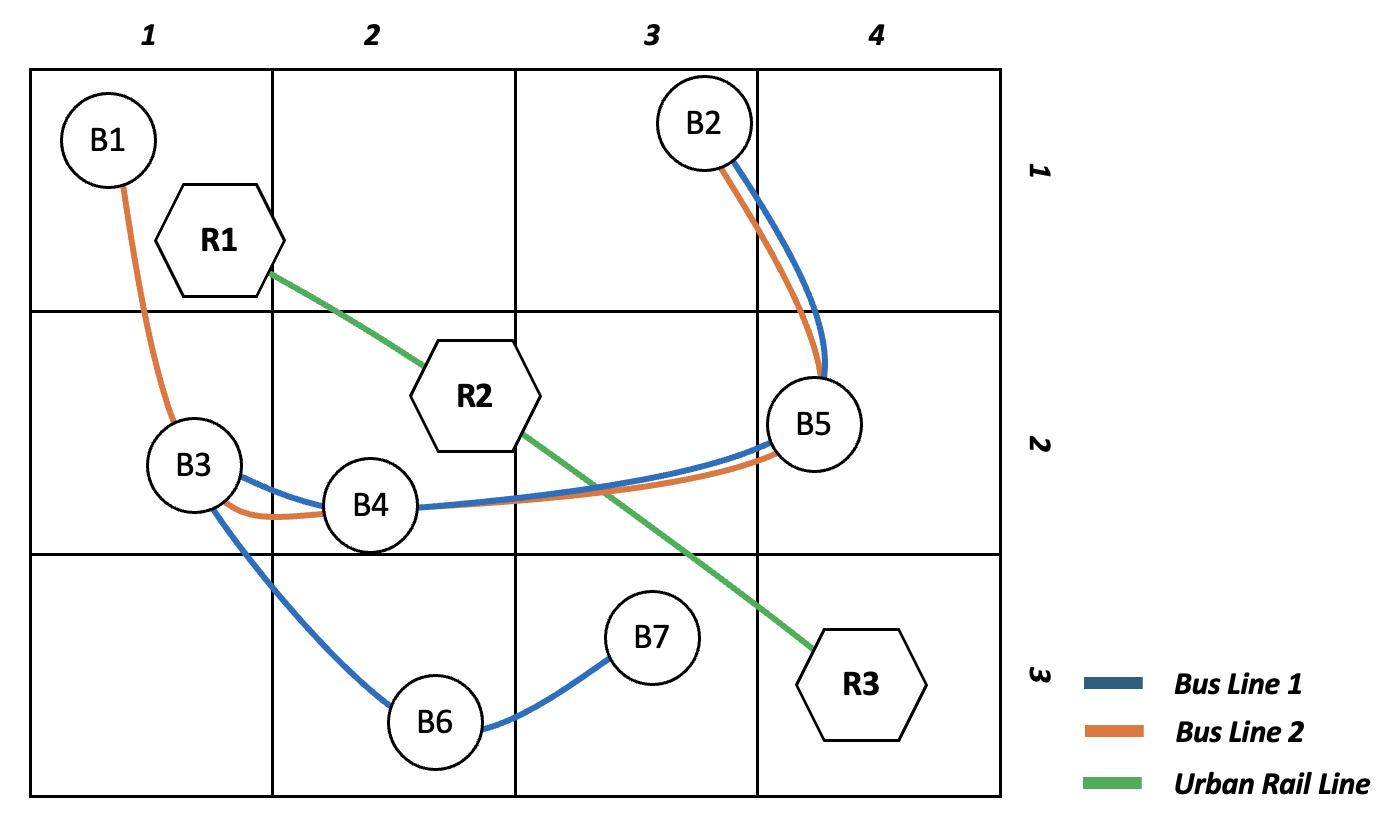
\includegraphics[width=\linewidth]{Figure/caseStudy.jpg}
\caption{Case study network: $3 \times 4$ tiles, rail stations R1--R3, bus stops B1--B7 and two bus lines.}\label{fig:case_illustration}
\end{minipage}\hfill
\begin{minipage}[c]{.41\textwidth}
\centering
\captionof{table}{Key parameters of the case study.}\label{tab:case_parameters}
\small
\begin{tabular}{@{}ll@{}}
\toprule
Parameter & Value \\
\midrule
Grid unit length & 2.0 km \\
Walking speed & 3.5 km/h \\
Bus speed & 25 km/h \\
Max.\ transfer walk time & 30 min \\
Rail frequency & 15 veh/h \\
Accessibility threshold $\tau$ & 30 min \\
\bottomrule
\end{tabular}
\end{minipage}
\end{figure}

Given a disruption scenario $\omega$, we compare four network states: the \emph{Nominal Baseline} $\pazocal G^O$ (intact network); the \emph{Unmitigated Disruption} $\pazocal G^\text{DISR}_\omega$, where disrupted rail segments are simply disabled; the \emph{Conventional Replacement Bus} $\pazocal G^\text{REPL}_\omega$, with additional buses operating along the disrupted rail link, which is the approach classically taken, although such buses travel on a road network with lower speed and higher circuity than the replaced rail; and \emph{Our Solution} $\pazocal G^\text{OURS}_\omega$, produced by model~\eqref{eq:obj}.

\textbf{Accessibility restoration.}\label{subsec:performance} We use two scenario-average indicators. The \emph{WA gain} is the relative improvement of accessibility compared with the disrupted network, $\overline{\Delta}^\text{gain}_{\text{WA}}(\omega;\pazocal G^\ast) = \frac{1}{|\pazocal S|}\sum_{s} \big(A_{s}(\pazocal G^\ast_\omega) - A_{s}(\pazocal G^\text{DISR}_\omega)\big)/A_{s}(\pazocal G^\text{DISR}_\omega)$. The \emph{opportunity change} $\overline{\Delta}^{\text{opp}}(\omega;\pazocal G^\ast) = \frac{1}{|\pazocal S|}\sum_{s} \big(N^{30}_{s,\omega}(\pazocal G^\ast) - N^{30}_{s,\omega}(\pazocal G^\text{DISR})\big)$ captures the variation in the number $N^{30}_{s,\omega}$ of opportunities reachable within 30 minutes.

\begin{table}[htbp]
\centering
\caption{Scenario-average performance: WA gains and 30-minute opportunity changes for the replacement bus and the optimized design.}
\label{tab:wa_scenarios}
\small
\begin{tabular*}{\textwidth}{@{\extracolsep{\fill}}lcccc@{}}
\toprule
Scenario & \multicolumn{2}{c}{WA Gain (tile avg.)} & \multicolumn{2}{c}{Opp.\ Change (tile avg.)}\\
\cmidrule(lr){2-3}\cmidrule(lr){4-5}
& Replacement Bus & Our Method & Replacement Bus & Our Method \\
\midrule
R1--R2 disrupted          & +11.92 & +12.15 & $-2.2$ & $-0.6$ \\
R2--R3 disrupted          & +11.30 & +12.13 & $-2.3$ & $-0.3$ \\
Both links disrupted      & +11.89 & +13.02 & $-3.0$ & $-1.3$ \\
\bottomrule
\end{tabular*}
\end{table}

Table~\ref{tab:wa_scenarios} reports the results. Across all disruption scenarios, both the replacement bus and the optimized design substantially improve accessibility, but the optimized design consistently achieves greater recovery. In terms of 30-minute reachability, both strategies incur average losses, confirming that the strict time threshold remains a binding constraint; however, the optimized design reduces these losses significantly relative to the replacement bus. By reallocating services toward time-critical OD pairs, our method delivers higher weighted accessibility while limiting the sacrifice of longer-distance opportunities.

\textbf{Proactive planning decisions.} We next examine the infrastructure measures made in advance of disruptions: which candidate stops to open and the extent to which the optimized bus network preserves the original line structure, measured by POPR (Table~\ref{tab:infra_decisions}).

\begin{table}[htbp]
\centering
\caption{Infrastructure decisions and line-structure preservation under different disruption scenarios (without dedicated lanes).}
\label{tab:infra_decisions}
\small
\begin{tabular*}{.75\textwidth}{@{\extracolsep{\fill}}lcc@{}}
\toprule
Scenario & Selected candidate stops ($z_i$) & POPR \\
\midrule
R1--R2 disrupted     & C1, C3, C4 & 1.000 \\
R2--R3 disrupted     & C1, C3     & 0.667 \\
Both links disrupted & C1, C3, C4 & 0.875 \\
\bottomrule
\end{tabular*}
\end{table}

Across scenarios, the model selects a small subset of stops (two or three out of four), while preserving much of the original line structure. When the R1--R2 link is disrupted, opening three stops achieves a POPR of 1.000, meaning the line order is fully retained. The R2--R3 disruption produces the most adjustment, with only two stops selected and a POPR of 0.667. Even with minimal infrastructure changes, the optimized design maintains high structural continuity, balancing adaptability with passenger familiarity.

% =============================================
\section{Conclusion and Future Work}\label{sec:conclusion}
% =============================================
This paper presented a proactive and adaptive optimization framework for improving the resilience of public transport systems during urban rail disruptions, with accessibility as the explicit objective. On a stylized case study built on a synthetic grid network, the proposed method consistently outperformed conventional bus-bridging strategies: it delivered larger gains in time-weighted accessibility and better preserved 30-minute reachability. Preparing only a small set of candidate bus stops in advance produced substantial benefits without materially altering the original line structure. These results underscore the value of jointly optimizing accessibility restoration and operational continuity when managing disruptions.

The present study is best regarded as a proof of concept. First, the framework should be applied to large-scale, real-world networks to assess its computational scalability and practical performance. Second, the current model does not fully capture the traffic dynamics induced by disrupted travel patterns, where reallocated demand can trigger congestion spillovers onto surrounding roads; incorporating such effects, for example through dedicated bus lanes and a spatially differentiated congestion response, is a natural next step.

\section*{Acknowledgements}
This work has been supported by the French ANR research project MuTAS (ANR-21-CE22-0025-01). We are grateful to the Gurobi Academic Program for providing Gurobi Optimizer.

\printbibliography

\end{document}
